\chapter{Grafika}
\thispagestyle{chapterBeginStyle}
\label{ch:graphics}

Ten rozdział traktuje o wy\'swietlaniu obiektów na ekranie i tworzeniu efektów specjalnych oraz cząsteczkowych.

Do wy\'swietlania grafiki w grze został użyty WebGL, rozwinięcie języka JavaScript, pozwalające wy\'wietlać obraz trójwymiarowy w przeglądarce. WebGL polega na używaniu shaderów, czyli programów wykonywanych na kartach graficznych. Język ten bazuje na języku OpenGL w wersji 2.0. WebGL jest tworzony przez Khronos Group, w skład którego wchodzą Mozilla, Apple, Google i Opera Software. W skład shaderów WebGL wchodzą dwa typy shaderów, vertex shader oraz fragment shader. Składnia jest podobna do języka C.\\
Typy danych dostępne w shaderach to:\begin{itemize}[topsep=0.2em, itemsep=0.5em, partopsep=0em, parsep=0em]
	\item bool, int i float, zachowujące się jak w zwykłym języku programowania
	\item \lbrack bi\rbrack vec2/vec3/vec4 - wektory wielko\'sci 2, 3 oraz 4 dla poprzednich typów - odpowiednio b to bool, i to int a brak przedrostka to float
	\item mat2/mat3/mat4 - macierze kwadratowe 2x2, 3x3, 4x4 ze zmiennymi typu float
	\item sampler2D - zmienna umożliwiająca dostęp do tekstury 2D
	\item samplerCube - zmienna umożliwająca dostęp do tekstury kostki
\end{itemize}
Można także używać struktur oraz tablicy zmiennych. W shaderach można także używać wielu funkcji matematycznych i geometrycznych, są tu także dostępne proste operacje na macierzach i wektorach jak mnożenie lub dodawanie.

Dostępne modyfikatory to:\begin{itemize}[topsep=0.2em, itemsep=0.5em, partopsep=0em, parsep=0em]
	\item const - podobnie jak w języku C, jest to stała, tylko do odczytu
	\item attribute - dostepne tylko w vertex shaderze - oznacza zmienną w której można umie\'scić dane przekazane do shadera (po podzieleniu)
	\item uniform - podobnie jak modyfikator attribute, ten modyfikator pozwala umie\'scić w zmiennej dane z zewnątrz, jednak tutaj są one wspólne dla wszystkich przetwarzanych wierzchołków, nie są dzielone, zazwyczaj są one używane do przekazania macierzy obrotu, przesunięcia lub perspektywy, oraz dostępu do tekstur
	\item varying - dane otrzymane z vertex shadera, które zostaną w przetworzone w rasteryzatorze i podane dalej do fragment shadera (można w nich umie\'scić np. pozycje wierzchołków na teksturze, a zostanie otrzymana pozycja dla każdego z pikseli w otrzymanym kształcie), nie może być strukturą
\end{itemize}

Zazwyczaj jako zmienne z modyfikatorem uniform przekazywane są macierze przekształceń oraz \'swiatła, z modyfikatorem attribute przekazywane są dane do shadera, a modyfikatora varying używa się dla danych przekazywanych z vertex shadera do pixel shadera, na przykład pozycja tekstury. 
Specyfikacja języka WebGL jest opisana na stronie Khronos Group\cite{WebGLSpecification}. Bardzo przydatny podczas pisania programów jest też krótki dokument opisujący w skrócie język WebGL\cite{WebGLReferenceCard}.\newpage

\noindent{\LARGE Vertex shader}\smallskip

Vertex shader zajmuje się przetwarzaniem wierzchołków. Dane są przekazywane w całości, i dzielone na poszczególne wierzchołki automatycznie. Na przykład, je\'sli do wektora składającego się z 4 pól podamy ciąg długości 12, to zostanie on podzielony na dane dla 3 wierzchołków.
Następnie procesor wydaje polecenia mówiące o tym które wierzchołki mają zostać przetworzone i jaki kształt ma zostać użyty. O tym które wierzchołki będą przetworzone decydujemy, wybierając pierwszy wierzchołek i ich ilo\'sć przy wywołaniu funkcji drawArrays(mode, first, count).
Dostępne kształty to:\begin{itemize}[topsep=0.2em, itemsep=0.5em, partopsep=0em, parsep=0em]
	\item punkty (każdy wierzchołek utworzy jeden punkt o zadanej wielko\'sci)
	\item linie, w tym:\begin{itemize}[topsep=0.2em, itemsep=0.5em, partopsep=0em, parsep=0em]
		\item pomiędzy parami wierzchołków (każda para tworzy osobną linię)
		\item łamana otwarta (linia jest utworzona między danym wierzchołkiem i następnym dla każdego z wybranych wierzchołków)
		\item łamana zamknięta (tak jak poprzednio, ale łączone są też pierwszy i ostatni wierzchołek)
	\end{itemize}
	\item trójkąty, w tym:\begin{itemize}[topsep=0.2em, itemsep=0.5em, partopsep=0em, parsep=0em]
		\item każda trójka wierzchołków osobno
		\item wachlarz (dla każdego wierzchołka poza pierwszym bierze się dany wierzchołek, następny wierzchołek oraz pierwszy wierzchołek)
		\item pas (brane są dany wierzchołek oraz dwa następne)
	\end{itemize}
\end{itemize}
Przykładowo można narysować dwa trójkąty podając dane dla 6 wierzchołków, ale jeśli te trójkąty mają wspólny bok to mozemy zmniejszyć ilość wierzchołków podając jedynie 4 rogi i rysując je jako wachlarz. Można w ten sposób zmniejszyć ilość danych wysyłanych do karty graficznej co przyspiesza program.

W pixel shaderze istnieje specjalna zmienna gl\_Position, do której należy zapisać pozycję wierzchołka po przetworzeniu, a także zmienna gl\_PointSize, służąca do ustawienia wielko\'sci punktu, je\'sli rysujemy punkty.\bigskip

\noindent{\LARGE Fragment shader}\smallskip

Fragment shader zajmuje się przetwarzaniem pojedynczych pikseli. Dane w tym shaderze otrzymuje się z rasteryzatora i są one osobne dla każdego piksela, który zostanie narysowany na ekranie. Po obliczeniu koloru danego fragmentu (lub odrzuceniu go), kolor zapisuje się w zmiennej gl\_FragColor. W tym shaderze dostępna są także zmienne gl\_FragCoord typu vec4, pozycja fragmentu na ekranie, oraz gl\_FrontFacing typu boolean, mówiąca czy powierzchnia danego fragmentu jest zwrócona w stronę kamery.

We fragment shaderze zazwyczaj na podstawie pozycji z tekstury i innych danych, takich jak pozycja, kolor i typ \'swiatła, oblicza się kolor danego piksela.\bigskip

\noindent Przykładowy kod prostego programu shader:\smallskip

{\large Vertex shader}
\begin{lstlisting}
attribute vec2 position;
attribute vec3 color;

varying vec3 c;

void main(void) {
	c = color;
	gl_Position = vec4(position, 0.0, 1.0);
	gl_PointSize = 10.0;
}
\end{lstlisting}\newpage

{\large Fragment shader}
\begin{lstlisting}
precision mediump float;
#define defaultAlpha 1.0

varying vec3 c;

void main(void) {
	gl_FragColor = vec4(c, defaultAlpha);
}
\end{lstlisting}
\begin{figure}[h]
	\centering
	\noindent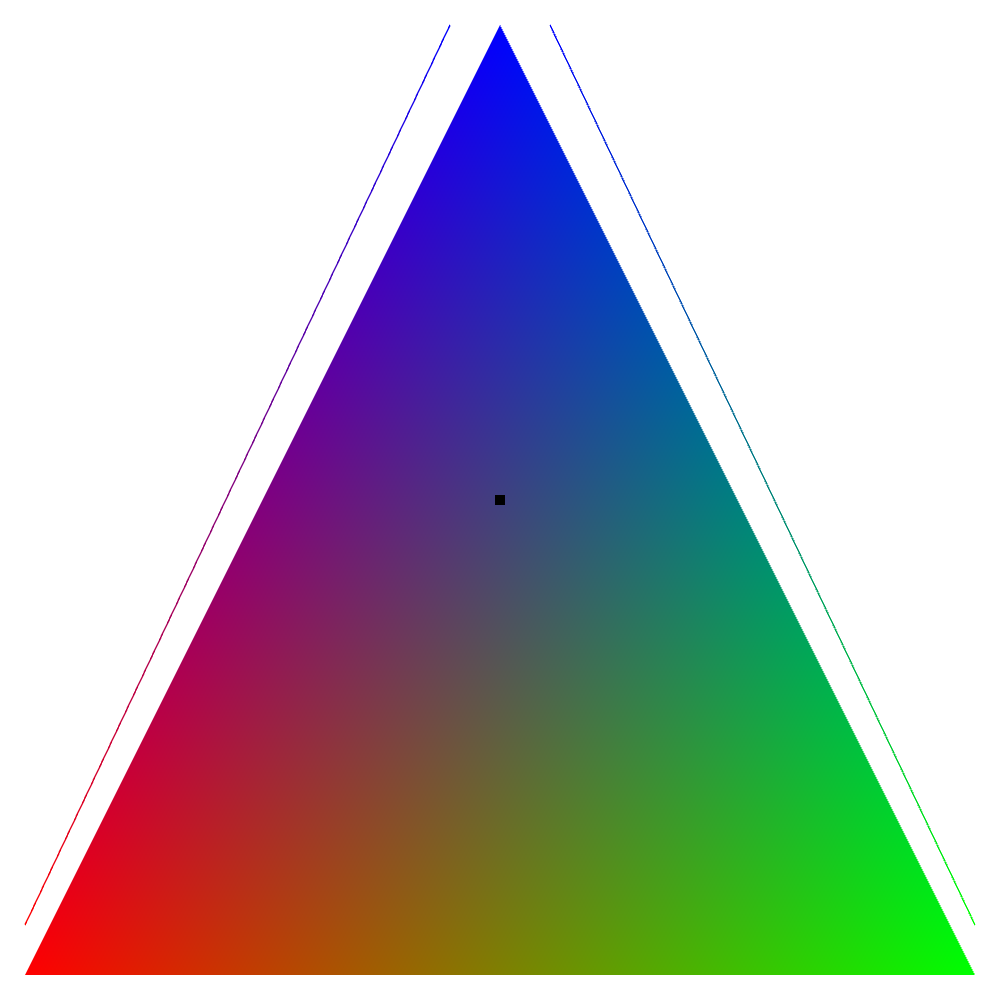
\includegraphics[width=\textwidth]{simple_shader}
	\caption{Wynik narysowania trójkąta, dwóch linii i punktu wielko\'sci 10 w przykładowym shaderze (szeroko\'sć punktu na ekranie to 10 pikseli)}
\end{figure}\vfill

\newpage\noindent{\LARGE Przykładowe shadery z efektami}

Zaprezentuję tutaj kilka shaderów tworzących ciekawe efekty. Można ich użyć jako efekty nałożone na całą scenę lub tylko no niektóre jej elementy, czasami też efekty same w sobie tworzą ładną grafikę.
Działają one w ten sposób, że kolor danego piksela jest obliczany jedynie na podstawie jego pozycji, używając funkcji matematycznych. Ze względu na działanie zostały podzielone na kształty oraz kolory.\bigskip

\noindent{\Large Kształty}

Kształty dają jako wynik liczbę, przez którą mnożymy kolor dla danego piksela, aby wzmocnić lub osłabić w nim kolor.\bigskip

\begin{wrapfigure}{l}{0.55\textwidth}
	\centering
	\noindent
\includegraphics[width=0.25\textwidth]{shape_rounded_square}
	\noindent
\includegraphics[width=0.25\textwidth]{shape_circles}
	\caption{Przykład zaokrąglonego kwadratu dla potęg 0.5, 1, 2 i 4 oraz efektu rozchodzących się kół}
\end{wrapfigure}

\noindent{\large Zaokrąglony kwadrat}

Uzyskuje się go przez obliczenie odległo\'sci za pomocą miary używającej innej potęgi (dla potęgi równej 2 uzyskuje się koło). Przy uzależnieniu stopnia potęgi od czasu można uzyskać ładny efekt pulsowania.\smallskip

\noindent{\large Rozchodzące się koła}

Ten efekt uzyskuje się przez pomnożenie odległo\'sci od \'srodka przez jaką\'s stałą, dodanie aktualnego czasu, a następnie użycie na wyniku funkcji okresowej, takiej jak sinus. Aby uzyskać efekt perpektywy i tunelu można też użyć logarytmu z odległo\'sci.\smallskip

\noindent{\large Pofalowane koło}

Efekt pofalowanego koła uzyskuje się przez obliczenie odległo\'sci od koła, którego promień zależy od kąta między danym punktem a \'srodkiem układu współrzędnych.\smallskip

\noindent{\large Fala}

Efekt fali uzyskuje się prze policzenie odległo\'sci od prostej, przesuniętej zależnie od wysoko\'sci.\smallskip

\noindent{\large Gwiazda}

Aby uzyskać efekt gwiazdy trzeba policzyć odległo\'sć od danego punktu w mierze o podstawie mniejszej niż 1, np. 0.3, przy wyższych potęgach uzyskuje się wypełniony zaokrąglony kwadrat.

\begin{figure}[h]
	\centering
	\noindent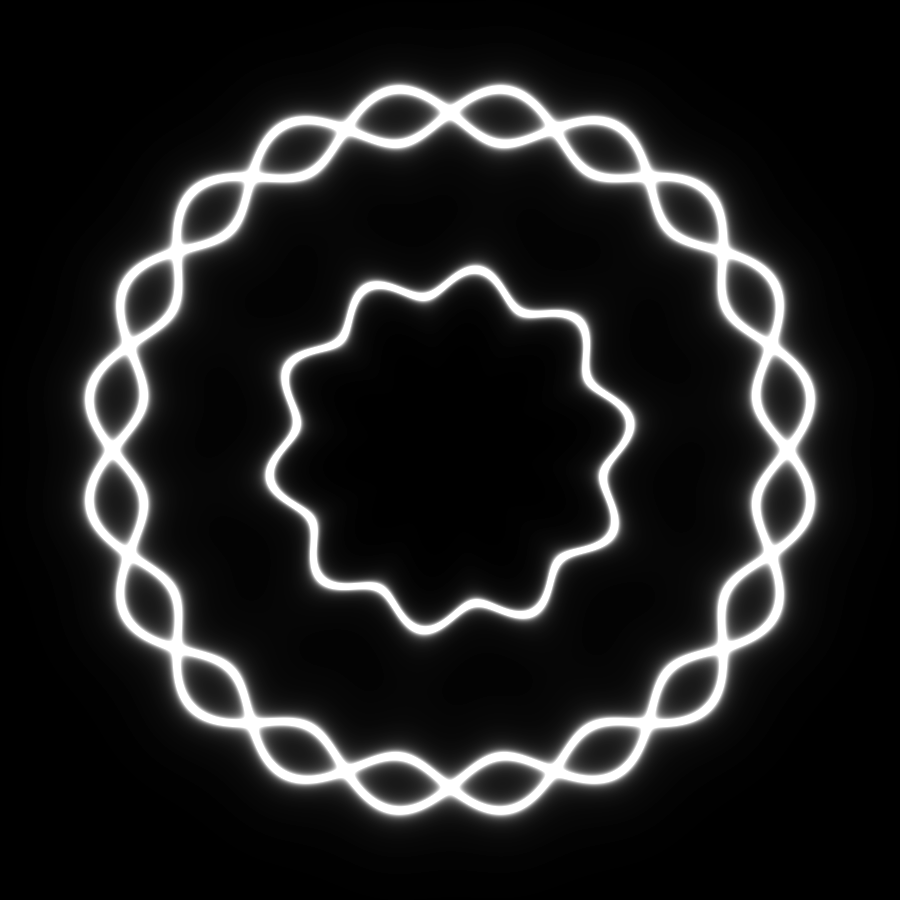
\includegraphics[width=0.3\textwidth]{shape_waved_circle}
	\noindent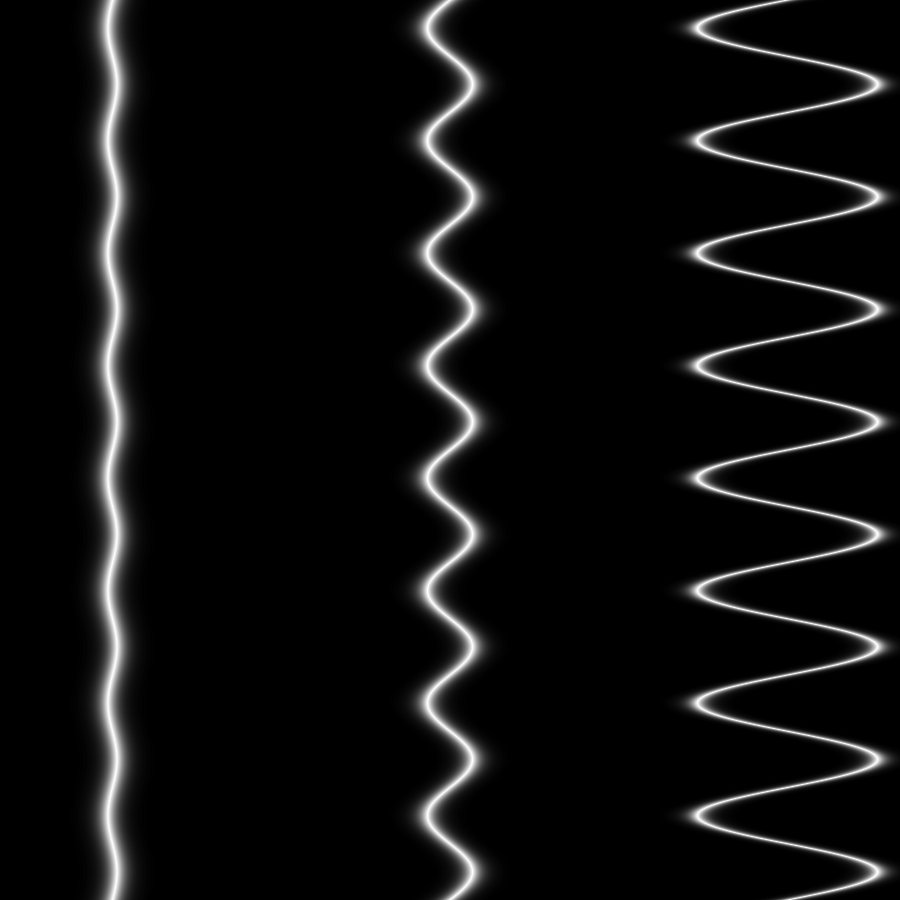
\includegraphics[width=0.3\textwidth]{shape_wave}
	\noindent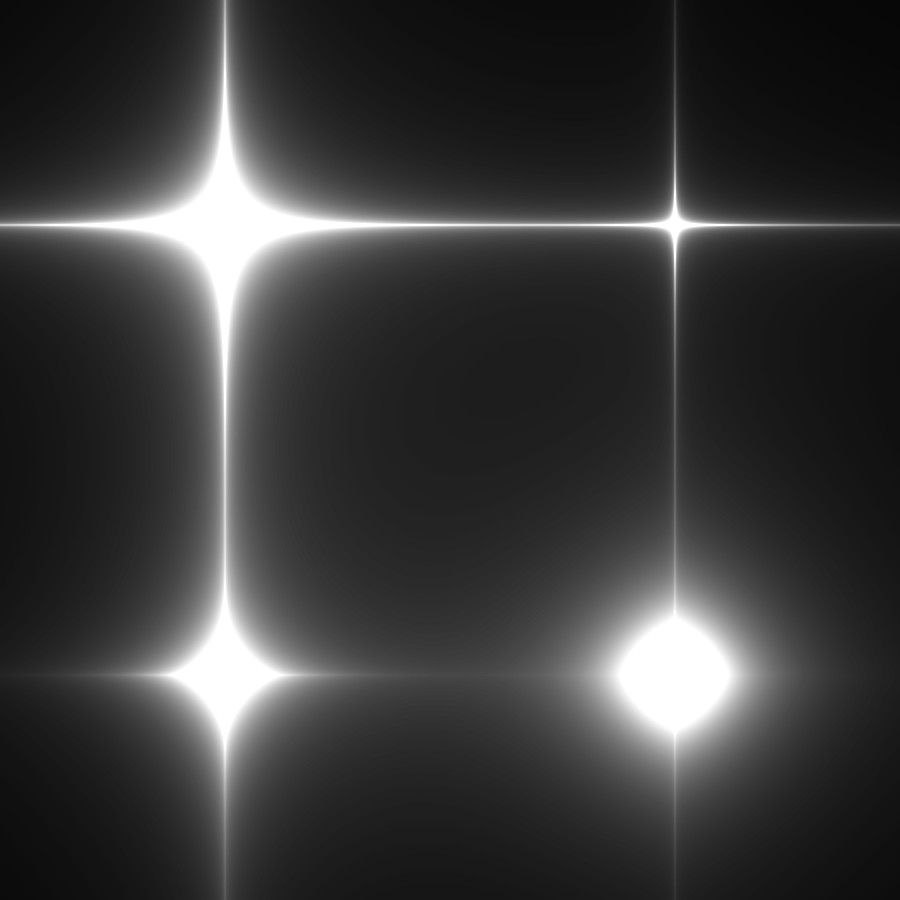
\includegraphics[width=0.3\textwidth]{shape_star}
	\caption{Przykład użycia efektów pofalowanego koła, fali oraz gwiazdy dla różnych danych}
\end{figure}\newpage

\noindent{\Large Kolory}

Kolory tworzą kolory zależnie od położenia, czasu oraz innych czynników. Można ich użyć żeby zmienić poszczególne barwy obrazu.

\noindent{\large Tęcza}

Efekt tęczy używa kąta do okre\'slenia siły poszczególnych kolorów we fragmencie.


\noindent{\large Disco}

Efekt disco używa odległo\'sci oraz kąta do okre\'slenia poszczególnych kolorów, może się także obracać obraz zmniejszać rozmiar. Poszczególne poziomy tego efektu (czyli fragmenty w różnych kolorach) moga poruszać się z różnymi prędko\'sciami. Można tak ustawić dane dla niego aby np. efekt zmniejszał się i zwiększał w rytm muzyki.

\begin{figure}[h]
	\centering
	\noindent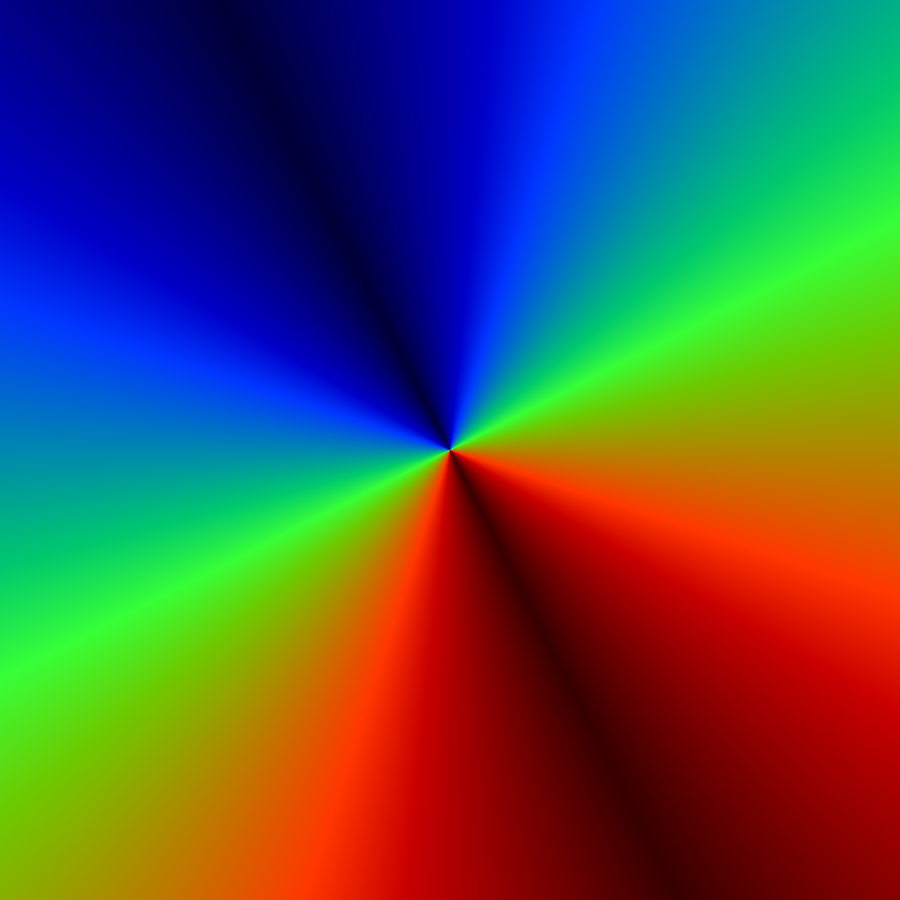
\includegraphics[width=0.49\textwidth]{color_rainbow}
	\noindent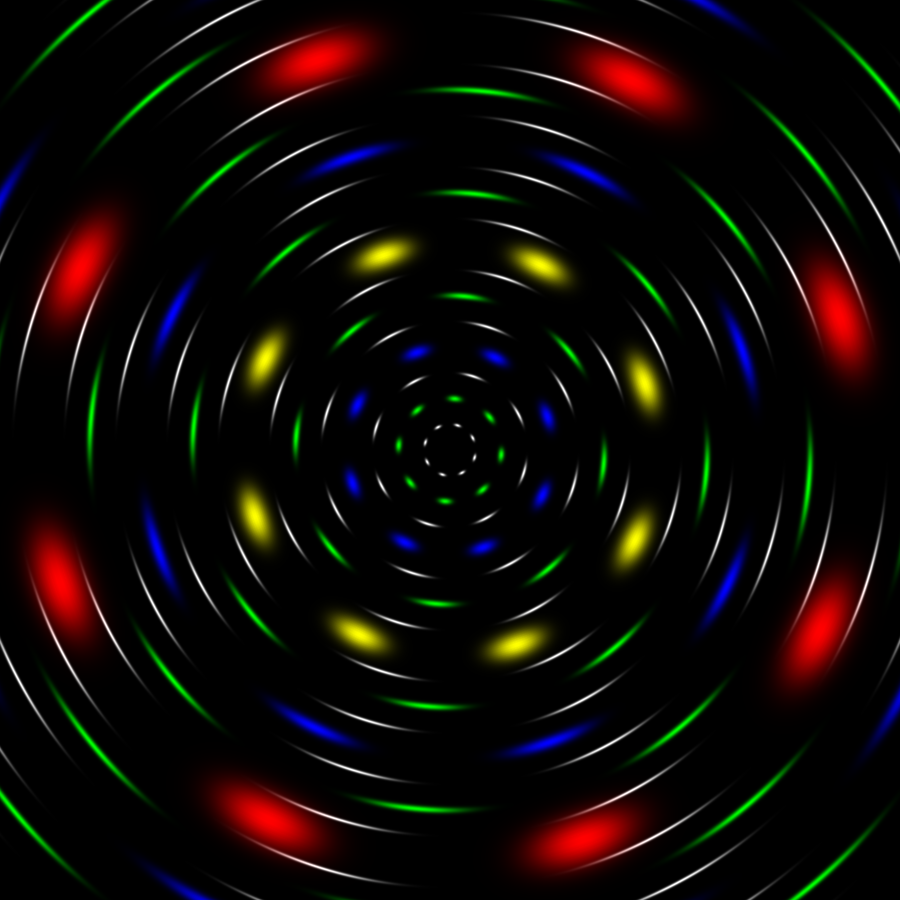
\includegraphics[width=0.49\textwidth]{color_disco}
	\caption{Przykład efektu tęczy oraz disco}
\end{figure}

Są także inne efekty, można na przykład poprzesuwać poszczególne kanały względem siebie, zmniejszyć ilo\'sć dostępnych kolorów, albo rozmyć obrazek. Aby uzykać ciekawsze efekty można też połączyć kształty z kolorami.
\begin{figure}[h]
	\centering
	\noindent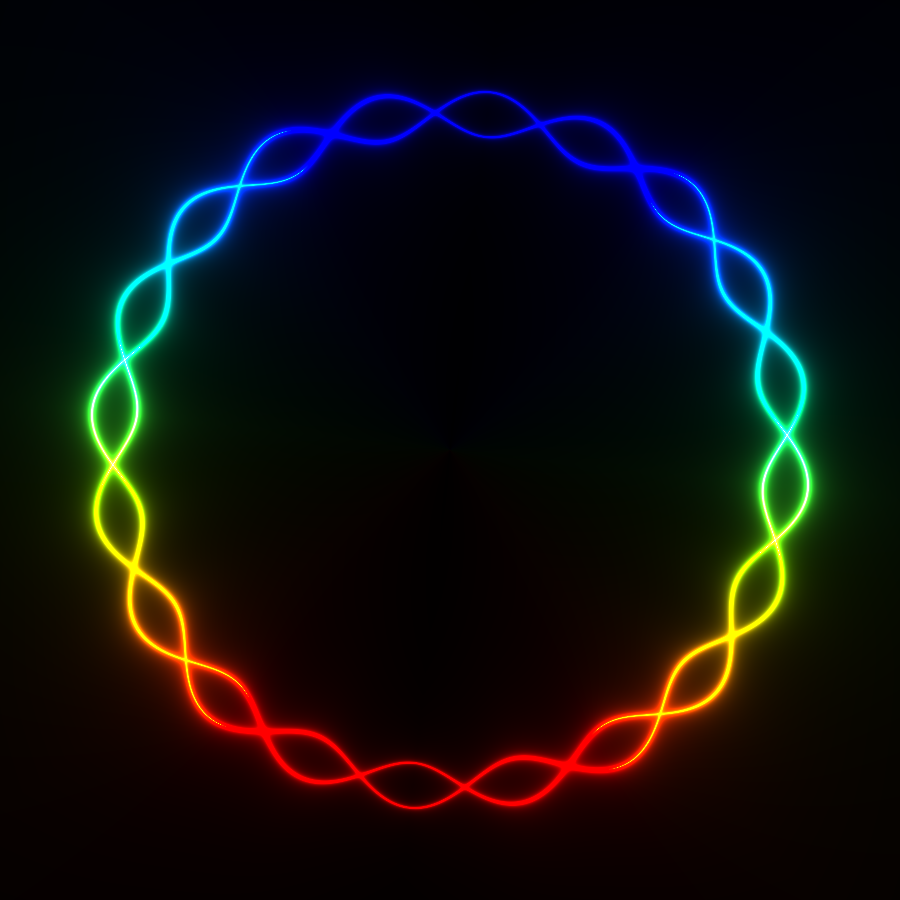
\includegraphics[width=0.425\textwidth]{effect0}
	\noindent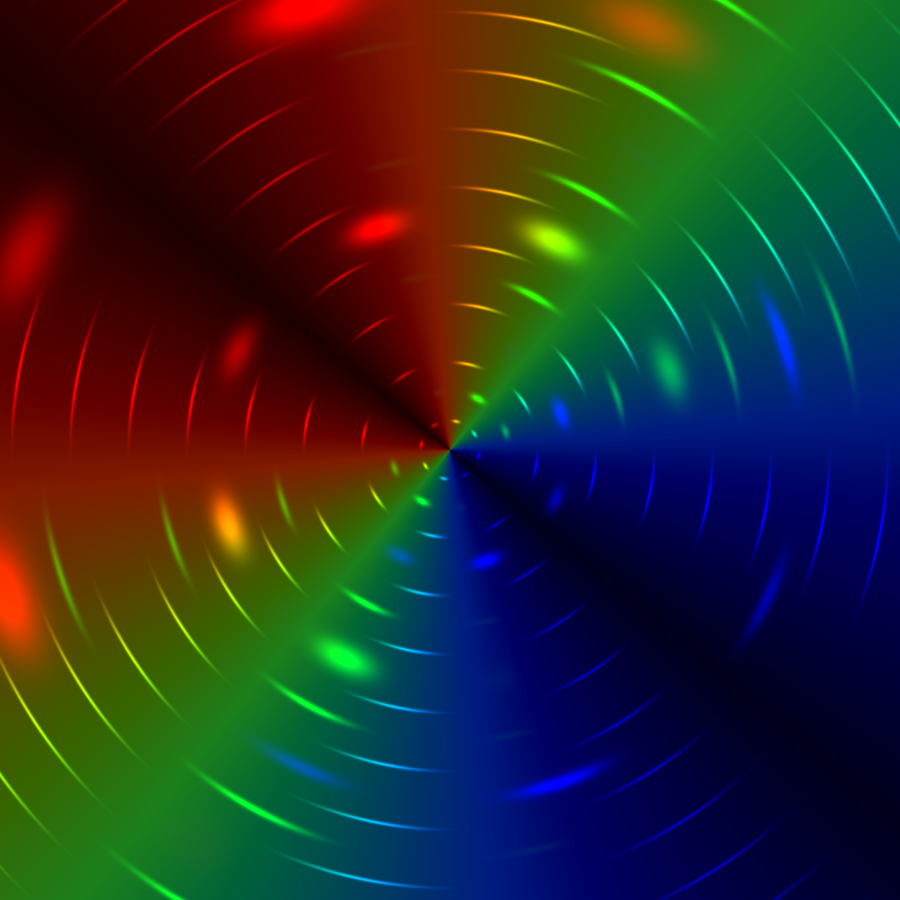
\includegraphics[width=0.425\textwidth]{effect1}
\end{figure}\newpage

\begin{figure}[h]
	\centering
	\noindent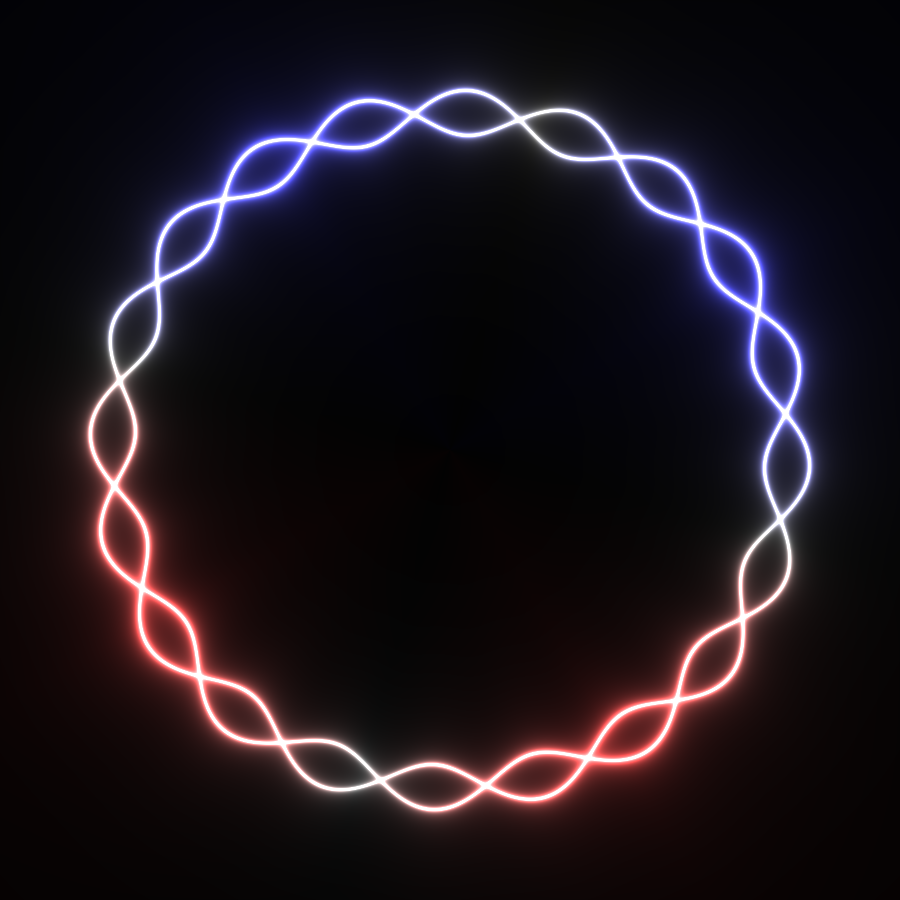
\includegraphics[width=0.495\textwidth]{effect2}
	\noindent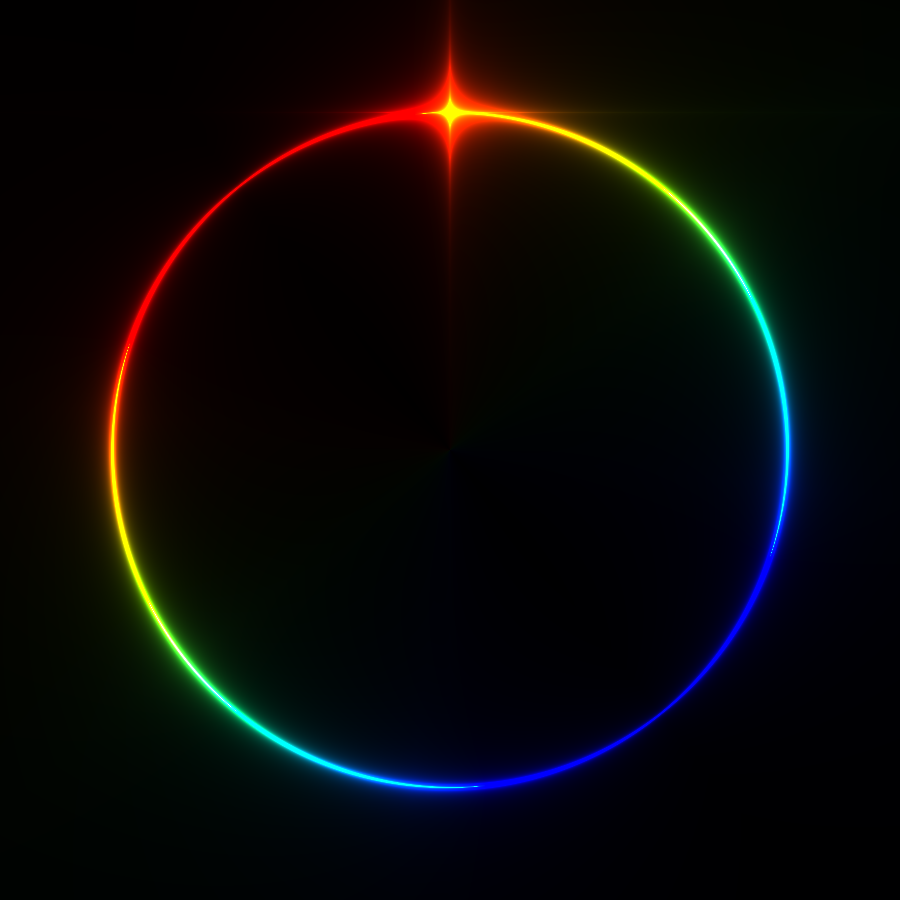
\includegraphics[width=0.495\textwidth]{effect3}
	\noindent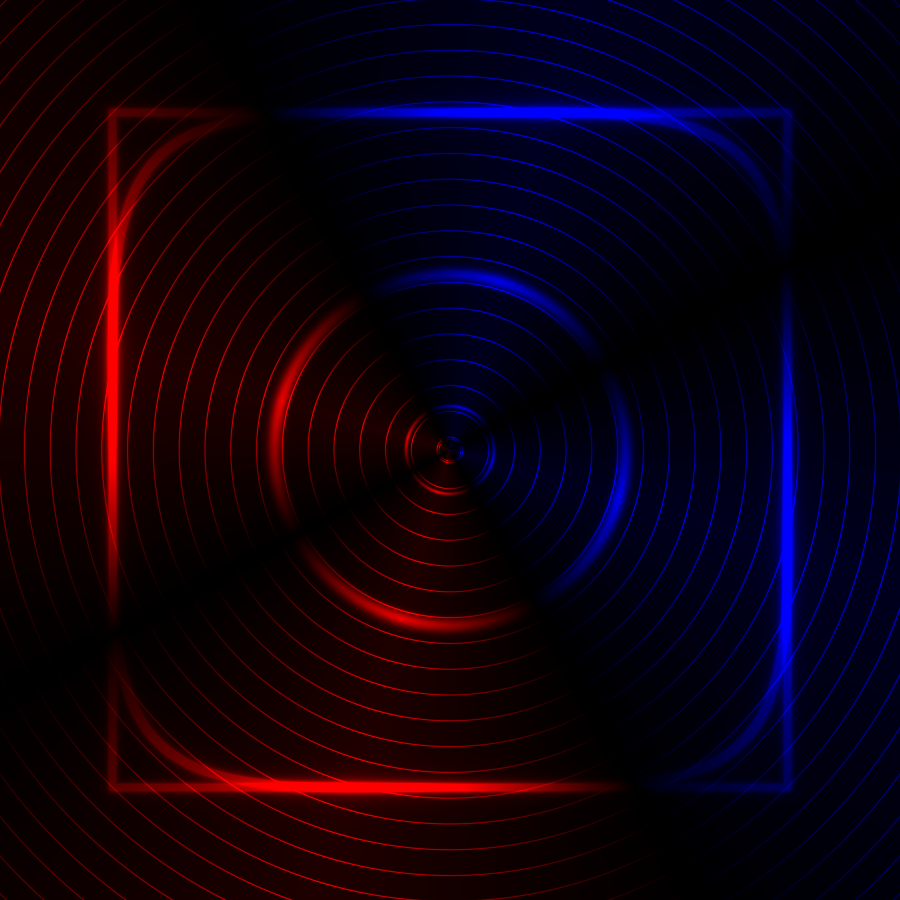
\includegraphics[width=0.495\textwidth]{effect4}
	\noindent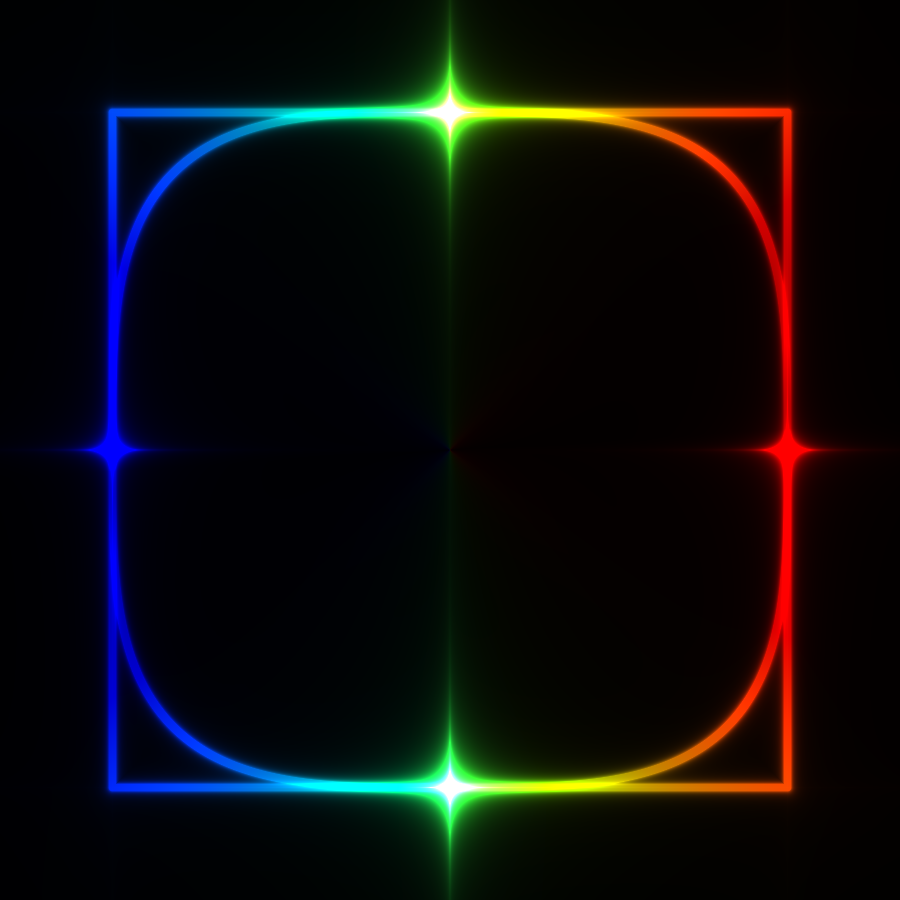
\includegraphics[width=0.495\textwidth]{effect5}
	\caption{Przedstawienie różnych efektów, powstałych przez połączenie różnych kształtów i kolorów}
\end{figure}\smallskip

\noindent Jak widać, efekty takie mogą bardzo ładnie wyglądać, chociaż wyglądają jeszcze lepiej w ruchu. 

Jednak same efekty zazwyczaj nie wystarczą w grze, potrzebne są też tekstury i obiekty, które trzeba narysować.\bigskip

{\LARGE Przygotowanie shaderów}\smallskip

Przedstawię teraz proces przygotowywania shaderów oraz danych dla nich. Pierwszym krokiem jest pobranie kontekstu dla elementu HTML Canvas, który jest wykorzystywany do rysowania. Aby to zrobić wystarczy użyć dostępnej dla obiektu Canvas funkcji getContext() i zapisaniu zwróconego obiektu do zmiennej (nazwijmy ją gl). To ten obiekt będzie podstawą do wykonywania wszelkich operacji, będziemy go używać do przesyłania danych, uruchamiania shaderów i rysowania.

Pierwszy krok to utworzenie buforów, które będą użyte do przesyłania danych do karty graficznej. Na razie bufory te będą nieprzypisane do żadnej ze zmiennych, nastąpi to dopiero po skompilowaniu shaderów.

Następny krok to wykorzystanie obiektu gl do stworzenia pustego shader programu. Potem tworzymy dwa shadery (typu vertex i typu fragment), ustawiamy jako ich kody źródłowe kody, które wcze\'sniej przygotowali\'smy w zmiennej typu string, i kompilujemy je. Po kompilacji obu shaderów możemy je przypiąć do naszego shader programu. Potem shader program zostaje uruchomiony przez użycie na obiekcie gl funkcji linkProgram(program) oraz useProgram(program). W dowolnym momencie można zmienić aktualnie używany shader program, należy jednak pamiętać aby wypełnić też wtedy na nowo bufory przypisane do danego programu.

Po uruchomieniu programu możemy wreszcie przypiąć bufory do zmiennych zawartych w naszych programach. Robi się to przez wyznaczenie danego bufora jako aktualnie używany, a następnie ustawienie mu wskaźnika na zmienną w dowolnym z shaderów. Przy przypisywaniu wskaźnika do bufora podaje się ile i jakie dane powinien on dostać na wej\'sciu. Na koniec należy jeszcze oznaczyć ten wskaźnik jako aktywny.

Należy zaznaczyć, że w ten sposób można przesyłać dane tylko do zmiennych z modyfikatorem attribute.

Kolejny krok to przygotowanie wskaźników na dane z modyfikatorem uniform. Wykonuje się to przez użycie funkcji getUniformLocation(program, nazwaZmiennej), która zwraca obiekt używany jako wskaźnik.

\noindent Przykładowy kod tworzący i łączący bufor colorBuffer ze zmienną color typu attribute vec3, a następnie pobierający wskaźnik zmiennej scale typu uniform float:
\begin{lstlisting}
var colorBuffer = gl.createBuffer();
gl.bindBuffer(gl.ARRAY_BUFFER, colorBuffer);
var colorLocation = gl.getAttribLocation(shader, "color");
gl.vertexAttribPointer(colorLocation, 3, gl.FLOAT, false, 0, 0);
gl.enableVertexAttribArray(colorLocation);
var scaleUniform = gl.getUniformLocation(shader, "scale");
\end{lstlisting}\bigskip

\noindent Drugi kod prezentuje sposób utworzenia wskaźnika do tekstury:
\begin{lstlisting}
var textureBuffer = gl.createTexture();
gl.uniform1i(gl.getUniformLocation(shader, "texture"), 0);
var img = new Image();
img.onload = (function(img) {
	return function() {
		gl.activeTexture(gl.TEXTURE0);
		gl.bindTexture(gl.TEXTURE_2D, textureBuffer);
		gl.texParameteri(gl.TEXTURE_2D, gl.TEXTURE_MAG_FILTER, gl.LINEAR);
		gl.texParameteri(gl.TEXTURE_2D, gl.TEXTURE_MIN_FILTER, gl.LINEAR);
		gl.texParameteri(gl.TEXTURE_2D, gl.TEXTURE_WRAP_S, gl.CLAMP_TO_EDGE);
		gl.texParameteri(gl.TEXTURE_2D, gl.TEXTURE_WRAP_T, gl.CLAMP_TO_EDGE);
		gl.texImage2D(gl.TEXTURE_2D, 0, gl.RGBA, gl.RGBA, gl.UNSIGNED_BYTE, img);
	};
})(img);
img.src = "texture.png";
\end{lstlisting}

Na początku zostaje stworzony bufor na teksturę, podobnie jak w przypadku zwykłego bufora. Następnie do zmiennej texture typu sampler2D zostaje przypisana warto\'sć 0, czyli pierwsza tekstura. na końcu zostaje utworzony obiekt typu Image, który po wczytaniu zadanego obrazka wrzuci go do bufora i ustawi wła\'sciwo\'sci tekstury. Około 85\% komputerów wspiera obecnie 16 jednostek tekstur. Ponadto 99,6\% komputerów wspiera tekstury o wielko\'sci maksymalnej co najmniej 4096x4096, a 50\% wspiera największą obecnie dostępną wielko\'sć tekstur - 16384x16384.

Należy też pamiętać, że w jednej teksturze można zawrzeć wiele różnych obrazów obiektów, do których będziemy się odwoływać przez pozycję na teksturze. Dzięki temu tekstury wystarczy zazwyczaj wczytać tylko raz, przy inicjalizacji.\newpage

\noindent Ostatni krok w przygotowaniu shadera do działania to ustawienie zmiennych takich jak:\begin{itemize}[topsep=0.2em, itemsep=0.5em, partopsep=0em, parsep=0em]
	\item używanie bufora głęboko\'sci - wtedy obiekty rysowane na ekranie nie mogą być nadrysowane przez te, które są za nimi
	\item funkcja głęboko\'sci - ustawienie testu głęboko\'sci (można na przykład ustawić, aby obiekt będący głębiej nadrysowywał te będące bliżej ekranu)
	\item viewport - ustawienie obszaru, na którym będziemy rysować
	\item używanie mieszania kolorów - decyduje czy kanał alfa będzie używany, aby połączyć kolory przy obiektach półprzezroczystych (je\'sli nie, będą one całkowicie wypełniać piksel)
	\item funkcja mieszania kolorów - decyduje w jaki sposób kolory będą mieszane
	\item stencil test - dodatkowy test, wykonywany dla każdego piksela w danej figurze, polega na porównaniu warto\'sci z bufora ze stałą za pomocą danej funkcji, można go użyć do nałożenia maski na wy\'swietlane elementy
\end{itemize}

Po przygotowaniu shader programu można użyć go do wy\'swietlania nim obiektów na ekranie. Aby wy\'swietlić co\'s, trzeba jednak włożyć dane do odpowiednich buforów. Aby włożyć dane, ponownie uaktywniamy dany bufor funkcją bindBuffer, a następnie używamy funkcji bufferData. Argumentem tej funkcji są dane, które zostaną podzielone i przypisane do poszczególnych wierzchołków. Podobnie zapisuje się dane w zmiennych typu uniform, używając wcze\'sniej przygotowanego wskaźnika.

Poniższy kod prezentuje umieszczanie danych w buforach:
\begin{lstlisting}
gl.uniform1f(scaleUniform, 1.5);
gl.bindBuffer(gl.ARRAY_BUFFER, colorBuffer);
gl.bufferData(gl.ARRAY_BUFFER, new Float32Array([1,1,1, 0,0,0]), gl.STREAM_DRAW);
\end{lstlisting}

Ponieważ dane dla colorBuffer-a to 6 liczb, a jest on przypisany do zmiennej składającej się z 3 liczb, zostaną one podzielone na dane dla dwóch wierzchołków.

Po przygotowaniu danych dla karty graficznej możemy wreszcie narysować scenę. Robi się to przez wywoływanie funkcji drawArrays, opisanej wcze\'sniej w tym rozdziale.\bigskip

\noindent{\LARGE \'Swiatło}

Do shaderów zostały dopisane funkcje obsługujące \'swiatło w grze. W projekcie zostały użyte 2 typy \'swiateł: punktowe, czyli \'swiecący punkt, oraz \'swiecąca linia, używane np. przy laserach.

Dane \'swiateł są przekazywane do shadera w zmiennych typu uniform. Dla każdego ze \'swiateł zostają przekazane odpowiednie dla niego dane:\begin{itemize}[topsep=0.2em, itemsep=0.5em, partopsep=0em, parsep=0em]
	\item dla \'swiateł punktowych zostają przekazane pozycja \'swiatła, kolor \'swiatła i kierunek oraz szeroko\'sć stożka \'swiatła
	\item dla \'swiatła będącego linią przekazywane są dane o kolorze, początku, długo\'sci i kącie pod jakim znajduje się prosta zawierająca dane \'swiatło
\end{itemize}

Na podstawie tych danych zostaje obliczony kolor \'swiatła padającego na dany obiekt w danym miejscu. Obliczenia zachodzą we fragment shaderze, dla każdego piksela osobno. Po policzeniu wszystkich \'swiateł zostaje dodane także \'swiatło otoczenia, o stałej warto\'sci niezależnie od położenia.

Ostateczne \'swiatło padające na dany punkt zostaje na koniec przemnożone przez kolor danego fragmentu, aby otrzymać końcowy kolor fragmentu.\bigskip

\noindent{\LARGE Shadery w grze}\smallskip

W grze istnieje kilka shaderów przeznaczonych do różnych zadań. Niektóre z nich służą do wy\'swietlania zwykłych tekstur, a inne do wy\'swietlania efektów specjalnych. Shadery są ułożone w odpowiedniej kolejno\'sci, tak aby najpierw rysowały się obiekty będące pod spodem, a nastepnie te będące na wierzchu. Wszystkie shadery znajdują się w tablicy, aby był do nich łatwy dostęp. Wszystkie shadery są obsługiwane przez obiekt klasy Graphics. Obiekt ten inicjalizuje wszystkie shadery, aktualizuje je, a także zawiera funkcje do przekazywania odpowiednich danych do każdego z shaderów w łatwy sposób. Dodatkowo obsługuje on też wysyłanie danych o \'swiatłach do każdego shadera, który je uwzględnia.

\cleardoublepage